\documentclass[Main]{subfiles}

\begin{document}


\section{Designprocess}

\subsection{Fjernbetjening}

Projektet skulle indeholde en sender som kunne sende kommandoer til dronen.

\begin{figure}[H]
\centering
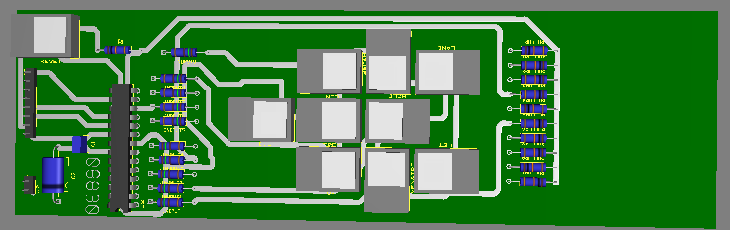
\includegraphics[width = 1 \textwidth]{3dUdenTal}
\caption{3D Figur af sender}
\label{Fig:3dUdenTal}
\end{figure}


Senderen er bygget op i form som en fjernbetjening for, at det er muligt at betjene den med én hånd.
Knapperne der er midt på printet er her brugeren giver sit input, som sendes videre.


\subsection{4+1 View}
Fjernbetjeningen udgør den største del af Use Casene beskrevet i kravspecifikationen\cite[s. 7 -- 11]{Kravspec}.

Et lille scenarie kunne optegnes og der kunne sættes nogle klasse navne på for, hvad der skulle være i de forskellige hardware-komponenter.

\begin{figure}[H]
\centering
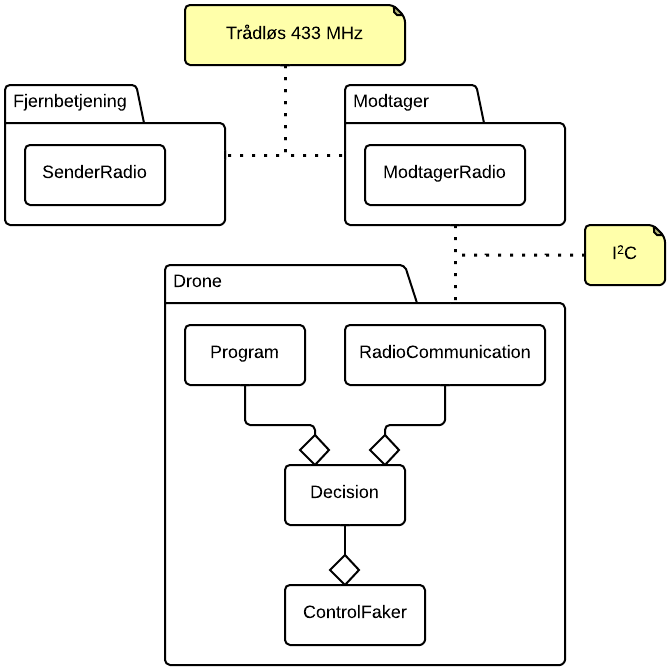
\includegraphics[width = 0.55 \textwidth]{Overview}
\caption{De første klasser}
\label{Fig:Overview}
\end{figure}


%Use Case 2 bliver brugt som eksempel for beskrivelsen af, hvordan systemet herefter blev udviklet.


\subsubsection*{Logic View}
Ved at analysere diagrammet yderligere med flere Use Cases, blev der optegnet flere klasser og til sidst var der et klassediagram. 
Fra klasse diagrammet blev små sekvensdiagrammet herefter udtænkt, således forbindelsen fra fjernbetjeningen til dronen blev mere håndgribelig, vist på Figur \ref{Fig:sendProgram}.

\begin{figure}[H]
\centering
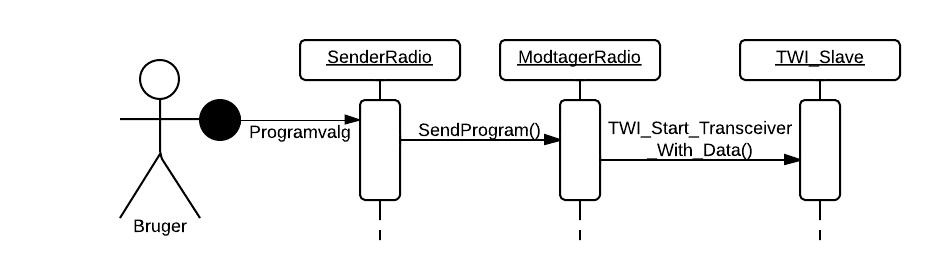
\includegraphics[width = 0.7 \textwidth]{SendProgram}
\caption{Sekvensdiagram fra fjernbetjening til drone.}
\label{Fig:sendProgram}
\end{figure}

\subsubsection*{Deployment View}
Da først der var noget funktionelt på hver enhed, blev kommunikationen imellem enhederne sat op.
Mellem fjernbetjeningen og modtageren skulle der være en 433 MHz forbindelse, som ville styre\dots\fxnote{RBK -- ace dette}

\subsubsection*{Process View}


\subsubsection*{Implementation View}
















\end{document}